\documentclass{beamer}
\usepackage{pgf,tikz}
%Module 1:
%Graphs and level sets, vector fields, the tangent space, surfaces, vector fields on surfaces, orientation.
%(Chapters 1 to 5 of \cite{thorpe}) (20 hours)
%Module 2:
%The Gauss map, geodesics, Parallel transport,
%(Chapters 6, 7 & 8 of \cite{thorpe}) (20 hours)
%Module 3:
%The Weingarten map, curvature of plane curves, Arc length and line integrals
%(Chapters 9, 10 & 11 of \cite{thorpe}) (25 hours)
%Module 4:
%Curvature of surfaces and Parametrized surfaces
%(Chapters 12 & 14 of \cite{thorpe}) (25 hours)

%Module 1 - \cite{thorpe} 1, 2, 3, 4, 5
%Module 2 - \cite{thorpe} 6, 7, 8
%Module 3 - \cite{thorpe} 9, 10, 11
%Module 4 - \cite{thorpe} 12, 14
%Missing - 13, 15, 16?
\title{Differential Geometry}
\author{Module I}
\institute{Chapter 1 : Level Sets and Graphs}

\begin{document}
\begin{frame}
\maketitle
\end{frame}

%\chapter{Graphs and Level Sets}
\section{Graphs and Level Set}
\begin{frame}{Level Set}
\begin{definition}
	Let function $f : U \to \mathbb{R}$ where $U \subset \mathbb{R}^{n+1}$.
	Let $c$ be a real number.
	Then the \textbf{Level set} of $f$ at height $c$ is the set of all points in $U$ with image $c$.
	\begin{equation}
		f^{-1}(c) = \{ (x_1,x_2,\cdots,x_{n+1}) \in U : f(x_1,x_2,\cdots,x_{n+1}) = c \}
	\end{equation} 
\end{definition}
\end{frame}

\begin{frame}{Graph}
\begin{definition}
	Let function $f : U \to \mathbb{R}$ where $U \subset \mathbb{R}^{n+1}$.
	Then,
\begin{equation}
	graph(f) = \{ (x_1,x_2,\cdots,x_{n+2}) \in \mathbb{R}^{n+2} : f(x_1,x_2,\cdots,x_{n+1}) = x_{n+2} \}
\end{equation}
\end{definition}

\begin{figure}[h]
	\centering
	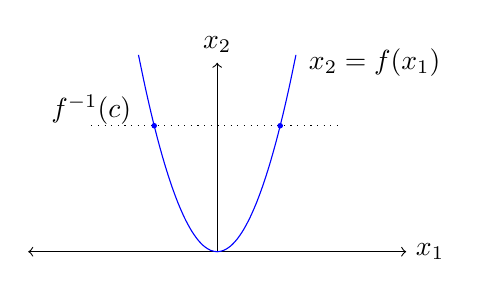
\begin{tikzpicture}[scale=0.8]
		\draw[<->] (-3, 0) -- (3, 0) node[right] {$x_1$};
  		\draw[->] (0, 0) -- (0, 3) node[above] {$x_2$};
  		\draw[scale=0.5, domain=-2.5:2.5, smooth, variable=\x, blue] plot ({\x}, {\x*\x});
		\draw[dotted,thin,black] (-2,2) -- (2,2);
		\draw (-2,2.25) node{$f^{-1}(c)$};
		\draw (2.5,3) node{$x_2 = f(x_1)$};
		\node[circle,fill=blue,inner sep=0pt, minimum size=2pt] at (1,2){};
		\node[circle,fill=blue,inner sep=0pt, minimum size=2pt] at (-1,2){};
\end{tikzpicture}
	\caption{Graph of $f(x_1)=x_1^2$ and Level set $f^{-1}(c)$}
\end{figure}
\end{frame}
\end{document}
